\begin{center}
\Huge
	Polær form
\end{center}
\section*{Komplekse tal på polær form}
\stepcounter{section}

Vi har set, at vi kan repræsentere komplekse tal som punkter i det komplekse plan. Idéen er nu, at vi vil repræsentere komplekse tal ud fra den vinkel, de danner med den reelle akse og deres afstand fra origo - det, vi kaldte modulus. 

\begin{setn}[Polær form]
	Et komplekst tal $z \in \mathbb{C}$ siges, at være på polær form, hvis 
	\begin{align*}
		z = r(\cos(\theta) + i \sin(\theta)).
	\end{align*}
	Tallet $r$ er modulus for $z$ og tallet $\theta$ kaldes \textit{argumentet} for $z$ og skrives Arg$(z)$.
\end{setn}
Er vores komplekse tal på formen $a + bi$, kan vi finde dets modulus og argument ved følgende formler.
\begin{align*}
	r &= |z| = \sqrt{a^2 + b^2}\\
	\theta &= \textnormal{Arg}(z) = \tan^{-1}\left(\frac{b}{a}\right)
\end{align*}
Det er selvfølgelig et krav i denne formel, at $a \neq 0$. 
Man skriver ofte forkortelsen $\textnormal{cis}(\theta)$ for $\cos(\theta) + i\sin(\theta)$. Betragter vi Figur \ref{fig:polær}, så kan vi se, hvorfor modulus og argument findes, som de gør. Vi har allerede set, at $|z|$ tilsvarer
afstanden fra (0,0) til det komplekse tal $z$ i det komplekse plan. Vi ser desuden, at realdelen Re$(z)$ og imaginærdelen
Im$(z)$ hver udgør en katete i en retvinklet trekant. Vi ved så fra trigonometri, at vinklen 
$\theta = \textnormal{Arg}(z)$ for det komplekse tal $a + bi$ kan findes ved formlen
\begin{align*}
	\tan(\theta) = \frac{b}{a} \ \Leftrightarrow \ \theta = \tan^{-1}\left(\frac{b}{a}\right).
\end{align*}
\begin{figure}[H]
	\centering
	\begin{tikzpicture}
	\begin{axis}[
	axis lines = center, 
	xmin = -2, xmax = 6,
	ymin = -2, ymax = 6, 
	ticks = none, 
	xlabel = Re, ylabel = Im,
	x = 1cm, y = 1cm,
	]
		\draw[color = white, thick] (axis cs: 0,0) -- (axis cs: 4,0);
		\draw[color = teal, thick] (axis cs: 0,0) -- (axis cs: 4,4) node[midway, anchor = south east] {$r = |z|$};
		\filldraw[color = teal] (axis cs: 4,4) circle (2pt) node[anchor = south west] {$z$};
		\draw[color = teal, thick, dashed] (axis cs: 4,0) -- (axis cs: 4,4) node[midway, anchor = west] {Im$(z)$};
		\draw[color = teal, thick, dashed] (axis cs: 0,0) -- (axis cs: 4,0) node[midway, anchor = north] {Re$(z)$};
		\draw[color = teal, thick] (axis cs: 0.5,0) arc[start angle = 0, end angle = 45, radius = 0.5cm] 
		node[midway, anchor = west, yshift = 2] {$\theta$};
	\end{axis}
	\end{tikzpicture}
	\caption{Komplekst tal repræsenteret ved argument $\theta$ og modulus $r$.}
	\label{fig:polær}
\end{figure}
Vi betragter et eksempel.
\begin{exa}
	Vi ønsker at repræsentere det komplekse tal $z = \sqrt{3} - i$ med polære koordinater. Vi indsætter i formlen og får
	\begin{align*}
		r = \sqrt{\sqrt{3}^2 + (-1)^2} = \sqrt{4} = 2.
	\end{align*}
	Vi har her fundet modulus $r = 2$. Vi finder nu argumentet Arg$(\sqrt{3}- i)$. Vi indsætter her tilsvarende i 
	formlen og får
	\begin{align*}
		\tan(\theta) = \frac{-1}{\sqrt{3}} = -\frac{\sqrt{3}}{3},
	\end{align*}
	og vi ved så, at $\theta = \frac{11\pi}{3}$. Vores komplekse tal lyder altså på polær form
	\begin{align*}
		z &= r(\cos(\theta) + i\sin(\theta)) \\
		&= 2\left(\cos\left(\frac{11\pi}{3}\right) + i\sin\left(\frac{11\pi}{3}\right)\right)\\
		&= 2\cis \left(\frac{11\pi}{3} \right)
	\end{align*}
\end{exa}
Det kan i disse opgaver være en fordel at anvende enhedscirklen på Figur \ref{fig:enhed} samt Tabel \ref{tab:trig}, som vi tidligere har set i vores trigonometriforløb.
\begin{figure}[H]
	\centering
	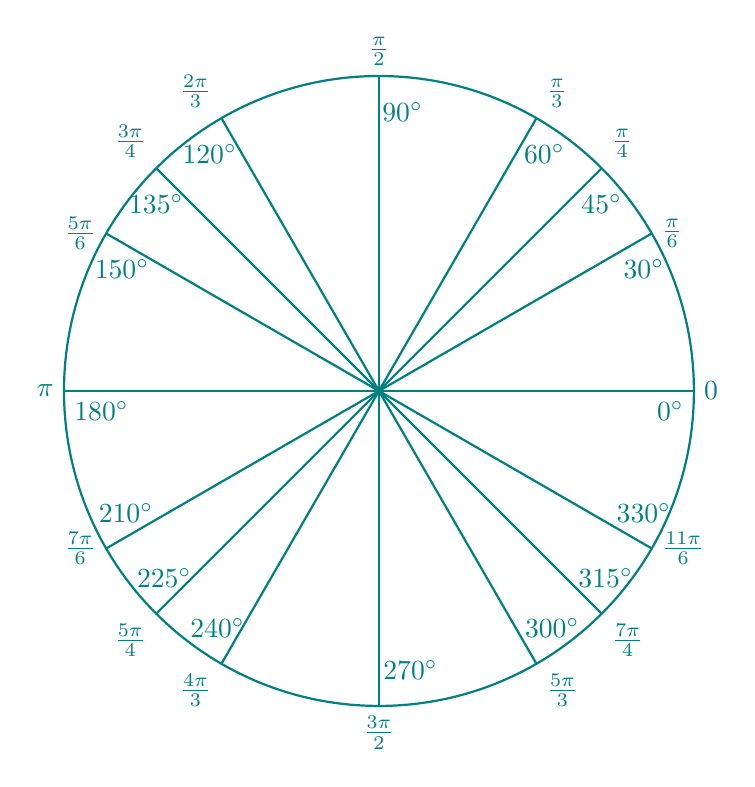
\begin{tikzpicture}
		\draw[thick, color = teal] (0,0) circle (4cm);
		\draw[thick, color = teal] (0,0) -- ({4*cos(0)},{4*sin(0)})
		node[pos = 1, anchor = north east] {$0^\circ$}
		node[pos = 1, anchor = west] {0};
		\draw[thick, color = teal] (0,0) -- ({4*cos(30)},{4*sin(30)})
		node[pos = 1, anchor = north, yshift = -0.2cm, xshift = -0.1cm] {$30^\circ$}
		node[pos = 1, anchor = west] {$\frac{\pi}{6}$};
		\draw[thick, color = teal] (0,0) -- ({4*cos(45)},{4*sin(45)})
		node[pos = 1, anchor = north, yshift = -0.2cm, xshift = -0cm] {$45^\circ$}
		node[pos = 1, anchor = south west] {$\frac{\pi}{4}$};
		\draw[thick, color = teal] (0,0) -- ({4*cos(60)},{4*sin(60)})
		node[pos = 1, anchor = north, yshift = -0.2cm, xshift = 0.1cm] {$60^\circ$}
		node[pos = 1, anchor = south west] {$\frac{\pi}{3}$};
		\draw[thick, color = teal] (0,0) -- ({4*cos(90)},{4*sin(90)})
		node[pos = 1, anchor = north, yshift = -0.2cm, xshift = 0.3cm] {$90^\circ$}
		node[pos = 1, anchor = south] {$\frac{\pi}{2}$};
		\draw[thick, color = teal] (0,0) -- ({4*cos(120)},{4*sin(120)})
		node[pos = 1, anchor = north, yshift = -0.2cm, xshift = -0.15cm] {$120^\circ$}
		node[pos = 1, anchor = south east] {$\frac{2\pi}{3}$};
		\draw[thick, color = teal] (0,0) -- ({4*cos(135)},{4*sin(135)})
		node[pos = 1, anchor = north, yshift = -0.2cm, xshift = -0cm] {$135^\circ$}
		node[pos = 1, anchor = south east] {$\frac{3\pi}{4}$};
		\draw[thick, color = teal] (0,0) -- ({4*cos(150)},{4*sin(150)})
		node[pos = 1, anchor = north, yshift = -0.2cm, xshift = 0.2cm] {$150^\circ$}
		node[pos = 1, anchor = east] {$\frac{5\pi}{6}$};
		\draw[thick, color = teal] (0,0) -- ({4*cos(180)},{4*sin(180)})
		node[pos = 1, anchor = north west] {$180^\circ$}
		node[pos = 1, anchor = east] {$\pi$};
		\draw[thick, color = teal] (0,0) -- ({4*cos(210)},{4*sin(210)})
		node[pos = 1, anchor = south, yshift = 0.2cm, xshift = 0.25cm] {$210^\circ$}
		node[pos = 1, anchor = east] {$\frac{7\pi}{6}$};
		\draw[thick, color = teal] (0,0) -- ({4*cos(225)},{4*sin(225)})
		node[pos = 1, anchor = south, yshift = 0.2cm, xshift = 0.1cm] {$225^\circ$}
		node[pos = 1, anchor = north east] {$\frac{5\pi}{4}$};
		\draw[thick, color = teal] (0,0) -- ({4*cos(240)},{4*sin(240)})
		node[pos = 1, anchor = south, yshift = 0.2cm, xshift = -0.05cm] {$240^\circ$}
		node[pos = 1, anchor = north east] {$\frac{4\pi}{3}$};
		\draw[thick, color = teal] (0,0) -- ({4*cos(270)},{4*sin(270)})
		node[pos = 1, anchor = south, yshift = 0.2cm, xshift = 0.4cm] {$270^\circ$}
		node[pos = 1, anchor = north] {$\frac{3\pi}{2}$};
		\draw[thick, color = teal] (0,0) -- ({4*cos(300)},{4*sin(300)})
		node[pos = 1, anchor = south, yshift = 0.2cm, xshift = 0.2cm] {$300^\circ$}
		node[pos = 1, anchor = north west] {$\frac{5\pi}{3}$};
		\draw[thick, color = teal] (0,0) -- ({4*cos(315)},{4*sin(315)})
		node[pos = 1, anchor = south, yshift = 0.2cm, xshift = 0.05cm] {$315^\circ$}
		node[pos = 1, anchor = north west] {$\frac{7\pi}{4}$};
		\draw[thick, color = teal] (0,0) -- ({4*cos(330)},{4*sin(330)})
		node[pos = 1, anchor = south, yshift = 0.2cm, xshift = -0.1cm] {$330^\circ$}
		node[pos = 1, anchor = west] {$\frac{11\pi}{6}$};
	\end{tikzpicture}
	\caption{Enhedscirklen med udvalgte vigtige vinkler.}
	\label{fig:enhed}
\end{figure}
\begin{table}[H]
	\centering
	\rowcolors{1}{SeaGreen!20}{Melon!20}
	\begin{tabular}{cccccc}
		$\theta$ & 0 & $\frac{\pi}{6}$ & $\frac{\pi}{4}$ & $\frac{\pi}{3}$ & $\frac{\pi}{2}$ \\
		$\cos(\theta)$ & 1 &  $\frac{\sqrt{3}}{2}$ & $\frac{\sqrt{2}}{2}$ & $\frac{1}{2}$ & 0 \\
		$\sin(\theta)$ & 0 & $\frac{1}{2}$ & $\frac{\sqrt{2}}{2}$ &  $\frac{\sqrt{3}}{2}$ & 1 \\
		$\tan(\theta)$ & 0 &  $\frac{\sqrt{3}}{3}$ & 1 & $\sqrt{3}$ & 
	\end{tabular}
	\caption{Vigtige funktionsværdier for cos, sin og tan.}
	\label{tab:trig}
\end{table}
\newpage
Det viser sig, at det er meget let at gange komplekse tal sammen, når de er på polær form. Vi har følgende sætning.
\begin{setn}\label{setn:gange}
	For to komplekse tal $z_1$ og $z_2$ givet ved
	\begin{align*}
		z_1 &= r_1(\cos(\theta_1) + i \sin(\theta_1))\\
		z_2 &= r_2(\cos(\theta_2) + i \sin(\theta_2))
	\end{align*}
	gælder der, at 
	\begin{align*}
		z_1z_2 = r_1r_2(\cos(\theta_1 + \theta_2) + i\sin(\theta_1 + \theta_2))
	\end{align*}
\end{setn}
Dette betyder altså, at man når man ganger to komplekse tal på polær form blot ganger modulus og lægger argumenterne sammen. 
\begin{exa}
	Lad $z_1$ og $z_2$ være givet ved følgende.
	\begin{align*}
		z_1 &= 2(\cos(3) + i \sin(3))\\
		z_2 &= 5(\cos(1) + i \sin(1))\\
	\end{align*}
	Så er $z_1z_2$ givet ved
	\begin{align*}
		z_1z_2 &= 2\cdot 5(\cos(3+1) + i \sin(3+1))\\
		 &= 10(\cos(4) + i \sin(4))\\
		 &= 10\textnormal{cis}(4)
	\end{align*}
\end{exa}
Det er dog værd at bemærke, at det kan være enddog ganske besværligt at lægge komplekse tal sammen, når de er på polær form. Det er det helt bestemt lettere at have dem i vores sædvanlige rektangulære koordinater.
\subsection*{Opgave 1}
Opskriv følgende komplekse tal i polære koordinater. 
\begin{align*}
	&1) \ i   &&2) \  1   &&3) \ 1 + i  \\
	&4) \ \frac{\sqrt{2}}{2} - \frac{\sqrt{2}}{2}i  &&5) \  \sqrt{3} + 3i   &&6) \  -1 + \sqrt{3}i \\
	&7) \ -\sqrt{3} -3i   &&8) \ -3 + 3\sqrt{3} i    &&9) \ 10 - 10i  \\ 
\end{align*}
 
\subsection*{Opgave 2}
Udregn følgende produkter af komplekse tal.

\begin{align*}
	&1) \  3\cis(2)\cdot 5\cis(4)  &&2) \ 1(\cos(3) + i \sin(3))\cdot 7(\cos(11) + i \sin(11))  \\
	&3) \  7\cis(5\pi/3)\cdot \cis(9\pi/5)  &&4) \ 2\cis(\pi/3)\cdot \cis(-3\pi/2)  \\
	&5) \  \sqrt{2}\cis(10\pi/11)\cdot \sqrt{2}\cis(15\pi/11) 
	 &&6) \ 13\cis(-11\pi/6)\cdot 15\cis(13\pi/3)  \\
\end{align*}

\subsection*{Opgave 3}

Udregn følgende potenser og rødder

\begin{align*}
	&1) \ (2\cis(3))^2  &&2) \ \sqrt{4(\cis(10))} \\
	&3) \ (\cis(\pi/2))^4  &&4) \ (\sqrt{7}\cis(-3))^4  \\
	&5) \  \sqrt[3]{27(\cis(9))} &&6) \  ((2\cis(4))^2)^5  \\
\end{align*}


\subsection*{Opgave 4}

Udnyt, at $\cos(v + w) =  \sin(v)\cos(w) - \cos(v)\sin(w)$ og $\sin(v + w) = \sin(v)\cos(v)-cos(v)\sin(w)$ til at vise Sætning \ref{setn:gange}.

\subsection*{Opgave 5}
Vi kalder et tal $z$ for en $n$'te enhedsrod, hvis $z^n = 1$. 
\begin{enumerate}[label=\roman*)]
	\item Kan du finde 2., 3., 4., 5. og 6. enhedsrødder. Tænk på enhedscirklen.
\end{enumerate}
 